\documentclass[paper=a4,fontsize=12pt]{scrartcl} % KOMA-article class

\usepackage[brazil]{babel}
\usepackage[utf8x]{inputenc}%Habilita acentuação
\usepackage[protrusion=true,expansion=true]{microtype}
\usepackage{amsmath,amsfonts,amsthm}     % Math packages
\usepackage{graphicx}                    % Enable pdflatex
\usepackage[svgnames]{xcolor}            % Colors by their 'svgnames'
\usepackage{geometry}
	\textheight=700px                    % Saving trees ;-)
\usepackage{url}

\frenchspacing              % Better looking spacings after periods
\pagestyle{empty}           % No pagenumbers/headers/footers

%%% Custom sectioning (sectsty package)
%%% ------------------------------------------------------------
\usepackage{sectsty}

\sectionfont{%			            % Change font of \section command
	\usefont{OT1}{phv}{b}{n}%		% bch-b-n: CharterBT-Bold font
	\sectionrule{0pt}{0pt}{-5pt}{3pt}}

%%% Macros
%%% ------------------------------------------------------------
\newlength{\spacebox}
\settowidth{\spacebox}{8888888888}			% Box to align text
\newcommand{\sepspace}{\vspace*{1em}}		% Vertical space macro

\newcommand{\MyName}[1]{ % Name
		\Huge \usefont{OT1}{phv}{b}{n} \hfill #1
		\par \normalsize \normalfont}

\newcommand{\MySlogan}[1]{ % Slogan (optional)
		\large \usefont{OT1}{phv}{m}{n}\hfill \textit{#1}
		\par \normalsize \normalfont}

\newcommand{\NewPart}[1]{\section*{\uppercase{#1}}}

\newcommand{\PersonalEntry}[2]{
		\noindent\hangindent=2em\hangafter=0 % Indentation
		\parbox{\spacebox}{        % Box to align text
		\textit{#1}}		       % Entry name (birth, address, etc.)
		\hspace{1.5em} #2 \par}    % Entry value

\newcommand{\SkillsEntry}[2]{      % Same as \PersonalEntry
		\noindent\hangindent=2em\hangafter=0 % Indentation
		\parbox{\spacebox}{        % Box to align text
		\textit{#1}}			   % Entry name (birth, address, etc.)
		\hspace{1.5em} #2 \par}    % Entry value

\newcommand{\EducationEntry}[4]{
		\noindent \textbf{#1} \hfill      % Study
		\colorbox{Black}{%
			\parbox{8em}{%
			\hfill\color{White}
			#2
			}} \par  % Duration
		\noindent \textit{#3} \par        % School
		\noindent\hangindent=2em\hangafter=0 \small #4 % Description
		\normalsize \par}

\newcommand{\WorkEntry}[4]{				  % Same as \EducationEntry
		\noindent \textbf{#1} \hfill      % Jobname
		\colorbox{Black}{\color{White}#2} \par  % Duration
		\noindent \textit{#3} \par              % Company
		\noindent\hangindent=2em\hangafter=0 \small #4 % Description
		\normalsize \par}

\usepackage{float}
\usepackage{wrapfig}

% sans-serif
%\renewcommand{\familydefault}{\sfdefault}

\begin{document}

	%%--------------------------------------------------------------------------
	%%% Photo
	%\begin{wrapfigure}{l}{0.5\textwidth}
	%	\vspace*{-2em}
	%		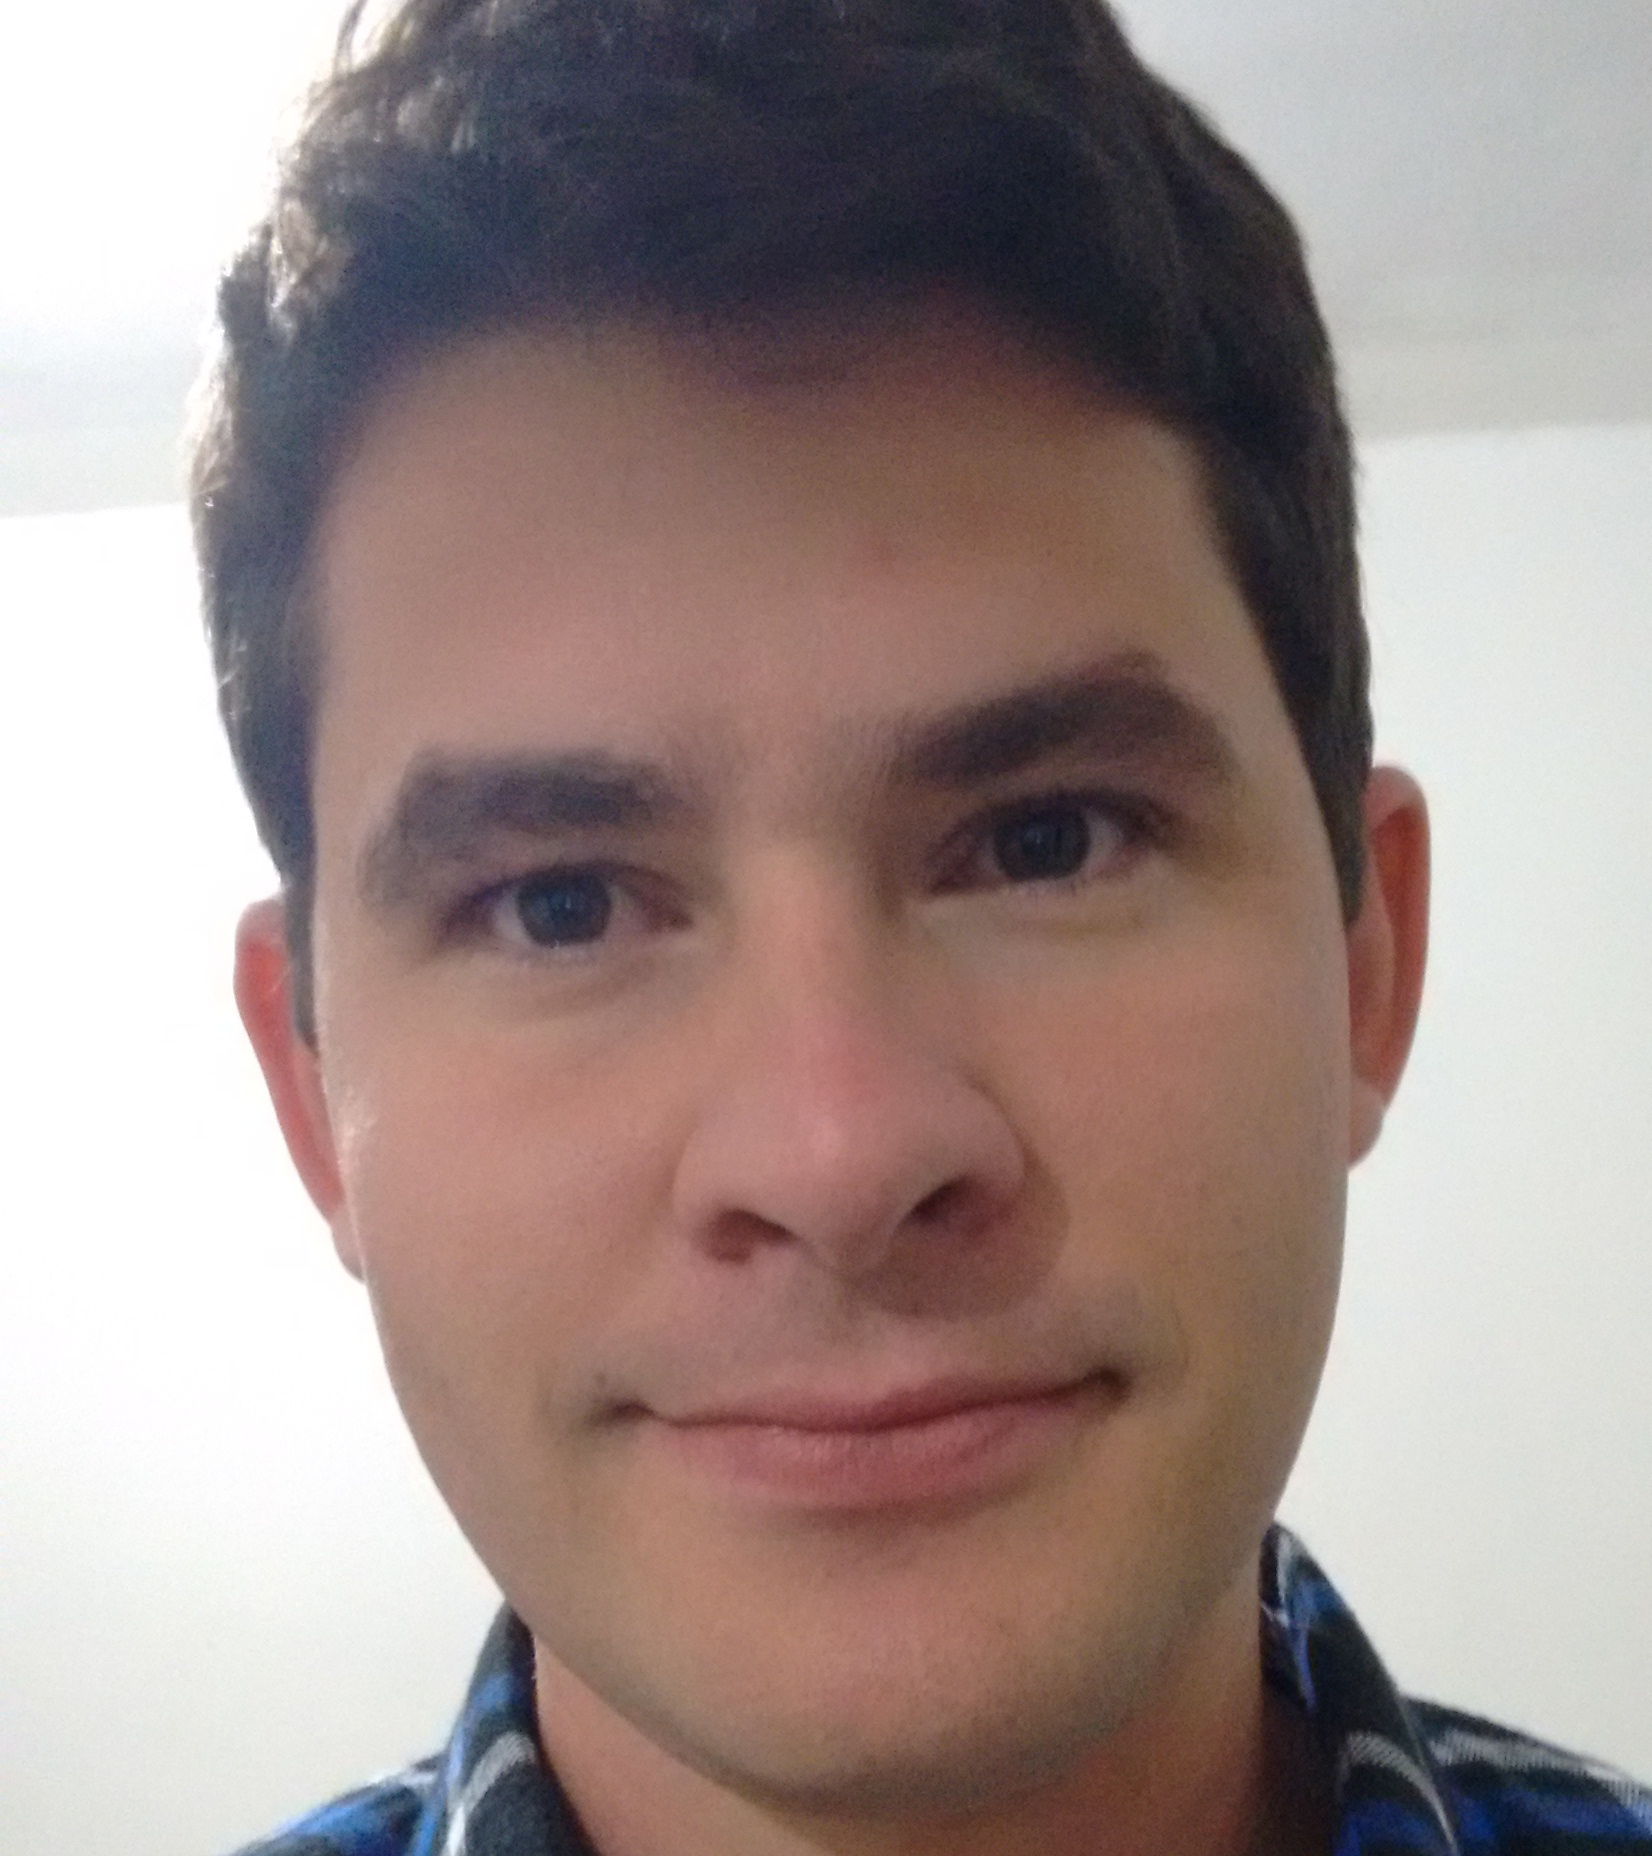
\includegraphics[width=0.15\textwidth]{images/perfil.jpg}
	%\end{wrapfigure}


	%%--------------------------------------------------------------------------
	\MyName{Ítalo Johnny}
	\MySlogan{Curriculum Vitae}
	\sepspace


	%%--------------------------------------------------------------------------
	\NewPart{Detalhes}{}
	\PersonalEntry{Nascimento}{23 de Março, 1989}
	\PersonalEntry{Cidade}{Franca, São Paulo}
	\PersonalEntry{Telefone}{(16)99108-5414, (16)3703-4911}
	\PersonalEntry{Email}{\url{italojohnnydosanjos@gmail.com}}
	\PersonalEntry{Linkedin}{\url{https://www.linkedin.com/in/italojohnny}}
	\PersonalEntry{Github}{\url{https://github.com/italojohnny}}


	%%--------------------------------------------------------------------------
	\NewPart{Experiência}{}
	\EducationEntry{Analista de Sistemas}
	{2017 - Atual\space\space\space\space}
	{JOYCAR - Carsharing., Período integral}
	{Desenvolvimento de firmware em Python para Linux embarcado, sobre a
	plataforma BeagleBone (ARM); Leitura de dados OBD dos veiculos; Comunicacao
	Socket; Desenvolvimento de firmware em C/C++ para microcontrolador, RFduino
	}
	\sepspace
	\EducationEntry{Técnico em redes Linux}
	{2015 - 2016\space\space\space\space}
	{FORIP - Tecnologia., Período integral}
	{Desenvolvimento e manutenção de sistema web, baseado no framework Python
	Web2py, integrado com serviço PABX Asterisk; Criação de extensão Firefox e
	Chrome para monitoramento de ramais e ligações; Elaboração de relatórios com
	Pentaho; Administração dos servidores Debian Asterisk; Atendimento aos clientes.
	}
	\sepspace
	%\EducationEntry{Estagiário}
	%{11/2014 - 12/2014}
	%{Enterplug Sistemas - Computer Systens., Meio período}{Suporte aos clientes dos
	%softwares da empresa; Desenvolvimento de aplição Web com framework Django.}
	%\sepspace
	\EducationEntry{Monitor de Informática}
	{2012 - 2014\space\space\space\space\space}
	{UNIFRAN - Universidade de Franca., Período integral}
	{Suporte aos setores acadêmicos da universidade; Criação e execução de rotinas
	de instalação de softwares; Manutenção dos computadores; Orientação dos
	estagiários nas tarefas do laboratório.}
	\sepspace
	\EducationEntry{Estagiário}
	{2011 - 2012\space\space\space\space\space}
	{UNIFRAN - Universidade de Franca., Meio período}
	{Auxilio de professores e alunos na utilização dos equipamentos e programas do
	laboratório.}


	%%--------------------------------------------------------------------------
	\NewPart{Educação}{}
	\EducationEntry{Mestrado em Ciência da Computação}{2016 - 
\includegraphics[scale=0.03]{images/padlock2.png} \space\space\space\space\space}
	{UFSCar - Universidade Federal de São Carlos.}
	{Linha de pesquisa: Sistemas de Automação e Robótica;\\
	Orientador: Prof. D.r. Orides Morandin Junior.}
	\sepspace
	\EducationEntry{Bacharelado em Ciência da Computação}{2011 - 2014\space\space\space\space\space}
	{UNIFRAN - Universidade de Franca}
	{TCC: OpenGL Aplicado ao Desenvolvimento de Jogos Eletrônicos;\\
	Orientador: Prof. M.e. Alysson Naves.}
	\sepspace
	\EducationEntry{Técnico em Informática}{2008 - 2009\space\space\space\space\space}
	{ETEC Dr. Júlio Cardoso}{}


	%%--------------------------------------------------------------------------
	\NewPart{Habilidades}{}
	\SkillsEntry{GNU/Linux}{Distribuições (Debian, Archlinux)}
	\SkillsEntry{}{}
	\SkillsEntry{Programacao}{C/C++ (STL, OpenGL, Allegro)}
	\SkillsEntry{}{Python (Django, Web2py)}
	\SkillsEntry{}{Bash, Javascript}
	\SkillsEntry{}{}
	\SkillsEntry{Ferramentas}{Git, Regex, SQL, Makefile, GDB7, Vim, UML, \LaTeX, Gnuplot}


	%%--------------------------------------------------------------------------
	\NewPart{Cursos}{}
	\EducationEntry{Raspberry Pi}{15h\space\space\space\space\space\space\space\space\space}
	{Introdução a sistemas embarcados, controle GPIO e servidor web.}{}
	\EducationEntry{Arduino}{20h\space\space\space\space\space\space\space\space\space}
	{Introdução e práticas em projetos com sensores e motores.}{}
	\EducationEntry{JmonkeyEngine}{5h\space\space\space\space\space\space\space\space\space}
	{Desenvolvimento de Jogos 3D em Java com JmonkeyEngine.}{}
	\EducationEntry{Introdução ao \LaTeX}{10h\space\space\space\space\space\space\space\space\space}
	{Linguagem de marcação para produção de textos matemáticos e físicos.}{}


	%%--------------------------------------------------------------------------
	%\NewPart{Idiomas}{}
	%\SkillsEntry{Português}{Nativo 	(Leitura, escrita e diálogo são fluentes)}
	%\SkillsEntry{Inglês}{Intermediário (Leitura e escrita são razoaveis)}
	%\SkillsEntry{Francês}{Intermediário	(Leitura e escrita são boas)}


\end{document}
